\documentclass[12pt, titlepage]{article}

\usepackage[pdftex]{graphicx}
\usepackage{booktabs}
\usepackage{tabularx}
\usepackage{hyperref}
\usepackage{float}
\usepackage{placeins}

\hypersetup{
    colorlinks,
    citecolor=black,
    filecolor=black,
    linkcolor=red,
    urlcolor=blue
}
\usepackage[round]{natbib}

\title{SE 3XA3: Test Report\\Mari0}

\author{Team 9, Ninetendo
		\\ David Hobson - hobsondd
		\\ Jose Miguel Ballesteros - ballesjm
		\\ Jeff Pineda - pinedaj
}

\date{\today}

%% Comments

\usepackage{color}

\newif\ifcomments\commentstrue

\ifcomments
\newcommand{\authornote}[3]{\textcolor{#1}{[#3 ---#2]}}
\newcommand{\todo}[1]{\textcolor{red}{[TODO: #1]}}
\else
\newcommand{\authornote}[3]{}
\newcommand{\todo}[1]{}
\fi

\newcommand{\wss}[1]{\authornote{blue}{SS}{#1}}
\newcommand{\ds}[1]{\authornote{red}{DS}{#1}}
\newcommand{\mj}[1]{\authornote{red}{MSN}{#1}}
\newcommand{\cm}[1]{\authornote{red}{CM}{#1}}
\newcommand{\mh}[1]{\authornote{red}{MH}{#1}}

% team members should be added for each team, like the following
% all comments left by the TAs or the instructor should be addressed
% by a corresponding comment from the Team

\newcommand{\tm}[1]{\authornote{magenta}{Team}{#1}}


\begin{document}

\maketitle

\pagenumbering{roman}
\tableofcontents
\listoftables
\listoffigures

\begin{table}[bp]
\caption{\bf Revision History}
\begin{tabularx}{\textwidth}{p{3cm}p{2cm}X}
\toprule {\bf Date} & {\bf Version} & {\bf Notes}\\
\midrule
2016-12-07 & 1.0 & Section 1,2,5,6,9\\
2016-12-08 & 1.0 & Section 4,7\\
\bottomrule
\end{tabularx}
\end{table}

\newpage

\pagenumbering{arabic}

\section{Functional Requirements Evaluation}

\subsection{Input Testing}

\begin{figure}[H]
   \centering
   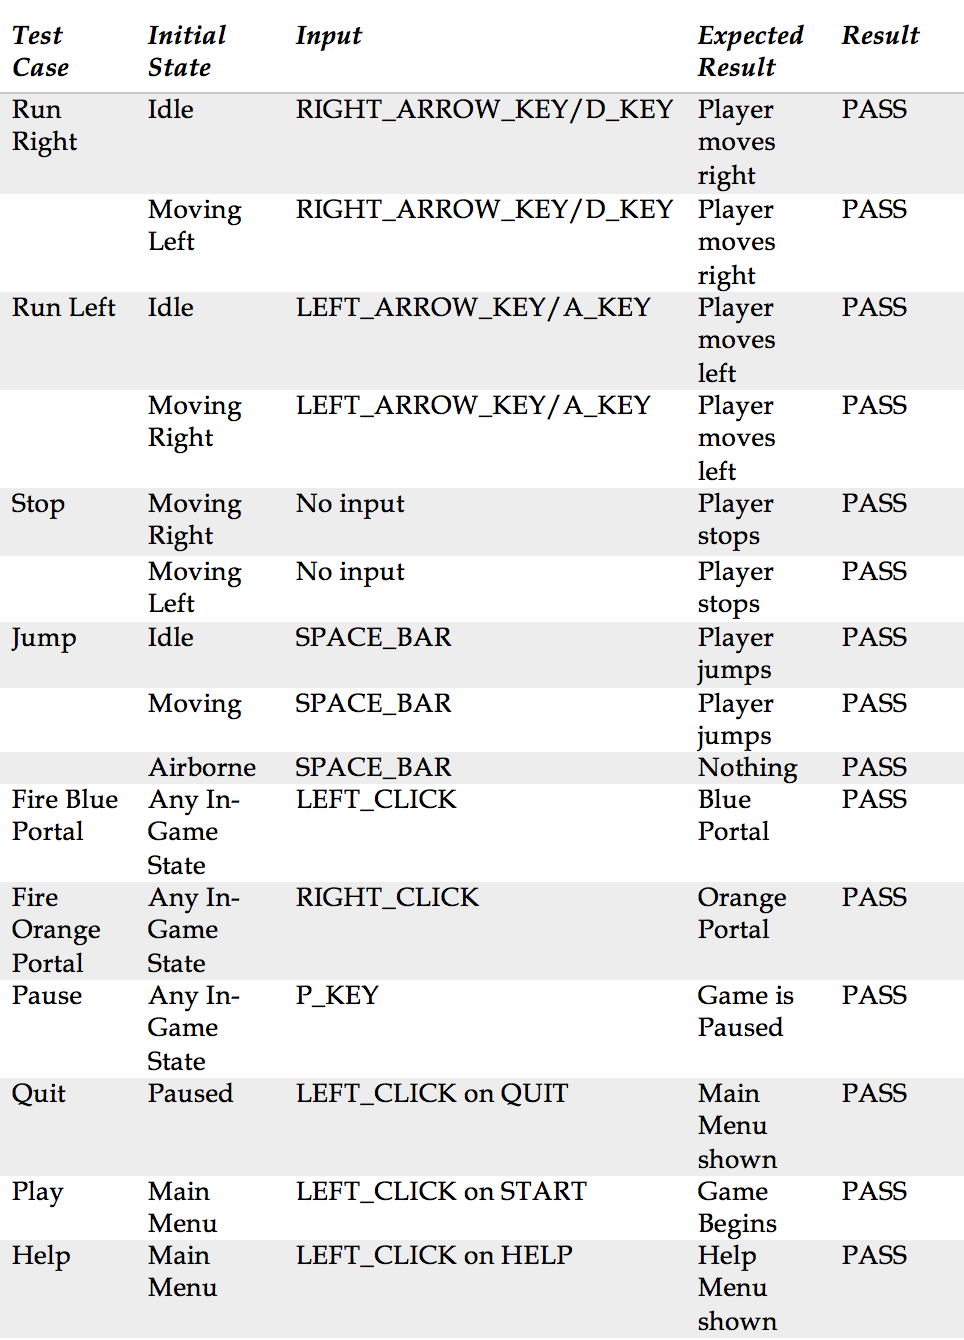
\includegraphics[scale=0.8]{Table1.png} % requires the graphicx package
   \label{fig:table1}
\end{figure}


\subsection{Collision Testing}

\begin{figure}[H]
   \centering
   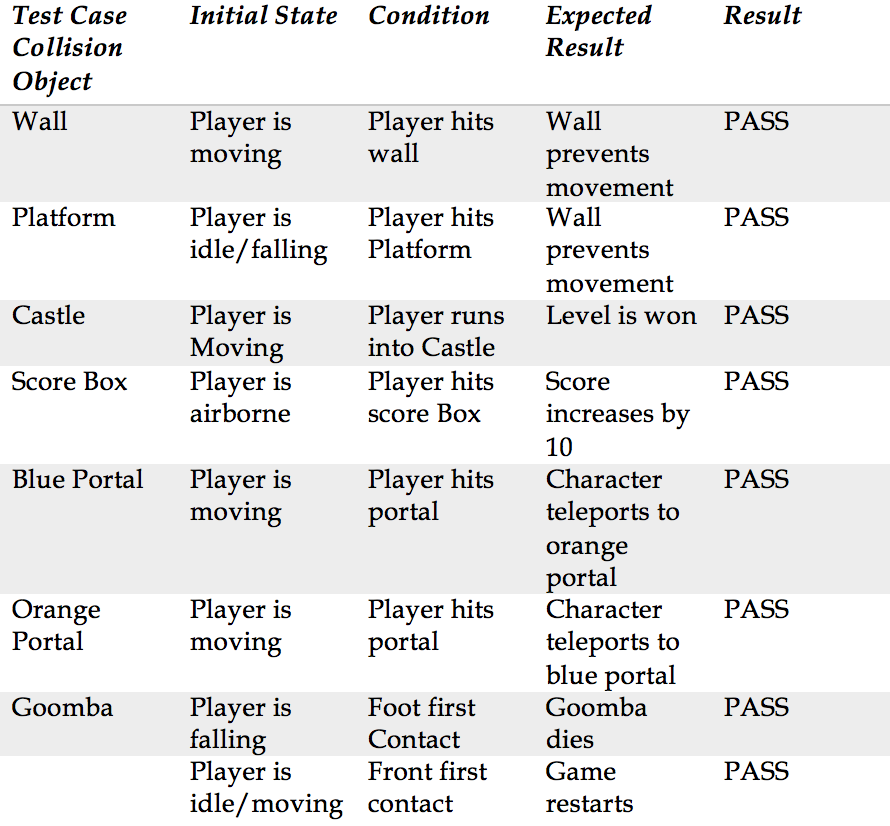
\includegraphics[scale=0.85]{Table2.png} % requires the graphicx package
   \label{fig:table2}
\end{figure}



\section{Nonfunctional Requirements Evaluation}

\textbf{Description:}
The following tests were executed by each member of our development team and a couple colleagues from our faculty. Engineering students were better suited for testing the current state of our project since it is an early development view of the open source game that is being recreated. Each participant was asked to give their honest feedback and suggestions.

\subsection{Look and Feel Requirements}

\begin{enumerate}

\item{Game Environment\\}

\textbf{Results: }All testers were able to explore all the game environments without issues.
					
\item{Game Hude/Interface\\}

\textbf{Results: }All testers stated that the location of the counter was not not obstructive in their opinion.

\end{enumerate}

\subsection{Usability and Humanity Requirements}

\begin{enumerate}

\item{Ease of Learning\\}

\textbf{Results: }All testers stated the game was easy to play and the controls were easy to learn.


\item{Entertainment\\}

\textbf{Results:} All testers stated that the game can be more enjoyable if it were stretched out to a longer period of time and had more gameplay, but is currently too short to provide a good amount of entertainment.

\end{enumerate}

\subsection{Performance Requirements}

\begin{enumerate}

\item{Controls/Commands\\}

\textbf{Results:} All testers noticed no delays or malfunction from the controls.

\end{enumerate}

\subsection{Operational and Environment Requirements}

\begin{enumerate}

\item{Operating System Support\\}

\textbf{Results:} Each tester was able to run the game on their own operating system. These include Windows and OSX 10.

\end{enumerate}

\subsection{Security Requirements}

\begin{enumerate}

\item{Altering Information\\}

\textbf{Results: }No tester indicated any type of alterations done to their current process or files.

\end{enumerate}


\subsection{Cultural Requirements}

\begin{enumerate}

\item{Spelling and Grammar\\}

\textbf{Results:} All testers indicated that the game had no spelling or grammar mistakes.

\item{Offensive Content\\}

\textbf{Results: }The testers indicated that they found no source of offensive content that would be directed at them or people from another culture.

\end{enumerate}

\subsection{Legal Requirements}

\begin{enumerate}

\item{License Adherence\\}

\textbf{Results: }The testers stated that they believe that the game is not breaching its current license.

\end{enumerate}

\subsection{Health and Safety Requirements}

\begin{enumerate}

\item{Epileptic Prevention\\}

\textbf{Results: }The testers indicated that they believe that the game would not trigger any epileptic seizures, although it is worth noting that non of the testers has ever had a history of epileptic seizures.

\end{enumerate}
	
\section{Comparison to Existing Implementation}	

This section will not be appropriate for every project.

\section{Unit Testing}

\begin{center}
\begin{tabular}{ | l | p{10cm} | }
\hline
Test Case Name &  TPG: Play Game Button	\\
Initial State &  User is viewing the main menu screen.	\\
Input & User left clicks the Play Game button	\\
Expected Results & User is taken to the game level and given control of Mario	\\
Actual Results &  User is taken to the game level and given control of Mario	\\
Test Result & Pass	\\
\hline
\end{tabular}
\end{center}

\begin{center}
\begin{tabular}{ | l | p{10cm} | }
\hline
Test Case Name & THP: Help Button	\\
Initial State & User is viewing the main menu screen	\\
Input & User left clicks the Help button	\\
Expected Results & User is taken to a screen that lists the controls of the game	\\
Actual Results & User is taken to a screen that lists the controls of the game	\\
Test Result & Pass	\\
\hline
\end{tabular}
\end{center}

\begin{center}
\begin{tabular}{ | l | p{10cm} | }
\hline
Test Case Name & TGP: Game Pause Functionality	\\
Initial State & User is in a level playing the game	\\
Input & The user presses down either the ESC key or the 'P' key on their keyboard	\\
Expected Results & The game is fully paused (game events no longer occur, user can no longer provide inputs, and audio stops).	\\
Actual Results & The game is fully paused.	\\
Test Result & Pass	\\
\hline
\end{tabular}
\end{center}

\begin{center}
\begin{tabular}{ | l | p{10cm} | }
\hline
Test Case Name & TST: In Game User Interface – Score Tracker	\\
Initial State & User is in a level playing the game	\\
Input & User increases their score by collecting coins or killing enemies	\\
Expected Results & Score increases by the value associated with coins and enemies	\\
Actual Results & Score increases by the value associated with coins and enemies	\\
Test Result & Conditional Pass (See next two unit test cases)	\\
\hline
\end{tabular}
\end{center}

\begin{center}
\begin{tabular}{ | l | p{10cm} | }
\hline
Test Case Name & TCCIS: Colleting Coins to Increase Score	\\
Initial State & User is in a level playing the game	\\
Input & User collects a coin by jumping from underneath and hitting a question mark block	\\
Expected Results & Score increases by a value of 10	\\
Actual Results & Score increases by a value of 10	\\
Test Result & Pass	\\
\hline
\end{tabular}
\end{center}

\begin{center}
\begin{tabular}{ | l | p{10cm} | }
\hline
Test Case Name & TKEIS: Killing Enemies to Increase Score	\\
Initial State & User is in a level playing the game	\\
Input & User lands on an enemy, killing the enemy \hspace*{4 in} \\
Expected Results & Score increases by a value of 50	\\
Actual Results & Score does not increase	\\
Test Result & Fail	\\
\hline
\end{tabular}
\end{center}

\begin{center}
\begin{tabular}{ | l | p{10cm} | }
\hline
Test Case Name & TKE: Killing Enemies	\\
Initial State & User is in a level playing the game	\\
Input & User lands on an enemy 	\\
Expected Results & Enemy is killed (removed from game)	 \hspace*{4 in}\\
Actual Results & Enemy is killed	\\
Test Result & Pass	\\
\hline
\end{tabular}
\end{center}

\begin{center}
\begin{tabular}{ | l | p{10cm} | }
\hline
Test Case Name & TDE: Dying to Enemies	\\
Initial State & User is in a level playing the game	\\
Input & User runs into an enemy (Player's current yvalue is less than or equal to Enemy's yvalue)	\\
Expected Results & Player is killed (removed from game) and game restarts the level	\\
Actual Results & Player is killed and player is placed at the beginning of the level	\\
Test Result & Pass	\\
\hline
\end{tabular}
\end{center}

\begin{center}
\begin{tabular}{ | l | p{10cm} | }
\hline
Test Case Name & TDF: Dying to Pit Fall	\\
Initial State & User is in a level playing the game	\\
Input & User falls into a pit fall (Falls off the screen)	\\
Expected Results & Player is killed (removed from game) and game restarts the level	\\
Actual Results & Player is killed and player is placed at the beginning of the level	\\
Test Result & Pass	\\
\hline
\end{tabular}
\end{center}

\begin{center}
\begin{tabular}{ | l | p{10cm} | }
\hline
Test Case Name & TFBVH: Firing a Blue Portal on a valid horizontal surface	\\
Initial State & User is in a level playing the game	\\
Input & Player left clicks on a horizontal surface that has enough space to fit the length of the portal	\\
Expected Results & A Blue Portal is placed horizontally on the surface	\\
Actual Results & A Blue Portal is placed horizontally on the surface	\\
Test Result & Pass	\\
\hline
\end{tabular}
\end{center}

\begin{center}
\begin{tabular}{ | l | p{10cm} | }
\hline
Test Case Name & TFBVV: Firing a Blue Portal on a valid vertical surface	\\
Initial State & User is in a level playing the game	\\
Input & Player left clicks on a vertical surface that has enough space to fit the length of the portal	\\
Expected Results & A Blue Portal is placed vertically on the surface	\\
Actual Results & A Blue Portal is placed vertically on the surface	\\
Test Result & Pass	\\
\hline
\end{tabular}
\end{center}

\begin{center}
\begin{tabular}{ | l | p{10cm} | }
\hline
Test Case Name & TFBNH: Firing a Blue Portal on a non-valid horizontal surface	\\
Initial State & User is in a level playing the game	\\
Input & Player left clicks on a horizontal surface that does not have enough space to fit the length of the portal	\\
Expected Results & A Blue Portal is not placed horizontally on the surface	\\
Actual Results & A Blue Portal is not placed horizontally on the surface	\\
Test Result & Pass	\\
\hline
\end{tabular}
\end{center}

\begin{center}
\begin{tabular}{ | l | p{10cm} | }
\hline
Test Case Name & TFBNV: Firing a Blue Portal on a non-valid vertical surface	\\
Initial State & User is in a level playing the game	\\
Input & Player left clicks on a vertical surface that does not have enough space to fit the length of the portal	\\
Expected Results & A Blue Portal is not placed vertically on the surface	\\
Actual Results & A Blue Portal is not placed vertically on the surface	\\
Test Result & Pass	\\
\hline
\end{tabular}
\end{center}

\begin{center}
\begin{tabular}{ | l | p{10cm} | }
\hline
Test Case Name & TFOVH: Firing an Orange Portal on a valid horizontal surface	\\
Initial State & User is in a level playing the game	\\
Input & Player right clicks on a horizontal surface that has enough space to fit the length of the portal	\\
Expected Results & An Orange Portal is placed horizontally on the surface	\\
Actual Results & An Orange Portal is placed horizontally on the surface	\\
Test Result & Pass	\\
\hline
\end{tabular}
\end{center}

\begin{center}
\begin{tabular}{ | l | p{10cm} | }
\hline
Test Case Name & TFOVV: Firing an Orange Portal on a valid vertical surface	\\
Initial State & User is in a level playing the game	\\
Input & Player right clicks on a horizontal surface that has enough space to fit the length of the portal	\\
Expected Results & An Orange Portal is placed vertically on the surface	\\
Actual Results & An Orange Portal is placed vertically on the 	\\
Test Result & Pass	\\
\hline
\end{tabular}
\end{center}

\begin{center}
\begin{tabular}{ | l | p{10cm} | }
\hline
Test Case Name & TFONH: Firing an Orange Portal on a non-valid horizontal surface	\\
Initial State & User is in a level playing the game	\\
Input & Player right clicks on a horizontal surface that does not have enough space to fit the length of the portal	\\
Expected Results & An Orange Portal is not placed horizontally on the surface	\\
Actual Results & An Orange Portal is not placed horizontally on the surface	\\
Test Result & Pass	\\
\hline
\end{tabular}
\end{center}

\begin{center}
\begin{tabular}{ | l | p{10cm} | }
\hline
Test Case Name & TFONV: Firing an Orange Portal on a non-valid vertical surface	\\
Initial State & User is in a level playing the game	\\
Input & Player right clicks on a vertical surface that does not have enough space to fit the length of the portal	\\
Expected Results & An Orange Portal is not placed vertically on the surface	\\
Actual Results & An Orange Portal is not placed vertically on the surface	\\
Test Result & Pass	\\
\hline
\end{tabular}
\end{center}

\begin{center}
\begin{tabular}{ | l | p{10cm} | }
\hline
Test Case Name & TMLS: Move Left when there is open space to the left of the character	\\
Initial State & User is in a level playing the game, player is grounded or in the air	\\
Input & Player presses the 'Left Arrow' key or the 'A' key	\\
Expected Results & Character's x velocity becomes negative and character is displaced to the left	\\
Actual Results & Character's x velocity becomes negative and character is displaced to the left	\\
Test Result & Pass	\\
\hline
\end{tabular}
\end{center}

\begin{center}
\begin{tabular}{ | l | p{10cm} | }
\hline
Test Case Name & TMRS: Move Right when there is open space to the right of the character	\\
Initial State & User is in a level playing the game, player is grounded or in the air	\\
Input & Player presses the 'Right Arrow' key or the 'D' key	\\
Expected Results & Character's x velocity becomes positive and character is displaced to the right	\\
Actual Results & Character's x velocity becomes positive and character is displaced to the right	\\
Test Result & Pass	\\
\hline
\end{tabular}
\end{center}

\begin{center}
\begin{tabular}{ | l | p{10cm} | }
\hline
Test Case Name & TMLNS: Move Left when there is no open space to the left of the character	\\
Initial State & User is in a level playing the game, player is grounded or in the air	\\
Input & Player presses the 'Left Arrow' key or the 'A' key	\\
Expected Results & Character's x velocity becomes zero and character is not displaced	\\
Actual Results & Character's x velocity becomes zero and character is not displaced	\\
Test Result & Pass	\\
\hline
\end{tabular}
\end{center}

\begin{center}
\begin{tabular}{ | l | p{10cm} | }
\hline
Test Case Name & TMRNS:  Move Right when there is no open space to the right of the character	\\
Initial State & User is in a level playing the game, player is grounded or in the air	\\
Input & Player presses the 'Right Arrow' key or the 'D' key	\\
Expected Results & Character's x velocity becomes zero and character is not displaced	\\
Actual Results & Character's x velocity becomes zero and character is displaced	\\
Test Result & Pass	\\
\hline
\end{tabular}
\end{center}

\begin{center}
\begin{tabular}{ | l | p{10cm} | }
\hline
Test Case Name & TJ: Jump	\\
Initial State & User is in a level playing the game and the character is grounded	\\
Input & Player presses the 'Up Arrow' key or the “W” Key	\\
Expected Results & Character's y velocity becomes positive and character is displaced upwards	\\
Actual Results & Character's y velocity becomes positive and character is displaced upwards	\\
Test Result & Pass	\\
\hline
\end{tabular}
\end{center}

\section{Changes Due to Testing}
After the testing was complete no urgent fixes that interfered with the requirements were needed to be made.

\section{Automated Testing}
No automated testing methods were used for the testing of this product.
		
\section{Trace to Requirements}
\begin{table}[!htbp]
\begin{tabular}{ll}
\toprule
Tests & Requirements \\
\midrule
TPG & R1 \\
THB & R1, R2 \\
TGP & R3 \\
TST & R4, R13 \\
TCCIS & R9, R13 \\
TKEIS & R11, R13 \\
TKE & R11 \\
TDE & R10 \\
TDF & R12 \\
TFBVH & R5 \\
TFBVV & R5 \\
TFBNH & R5 \\
TFBNV & R5 \\
TFOVH & R5 \\
TFOVV & R5 \\
TFONH & R5 \\
TFONV & R5 \\
TMLS & R6 \\
TMRS & R6 \\
TMLNS & R6 \\
TMRNS & R6 \\
TH & R7\\
\midrule
\end{tabular}
\caption{Trace between Tests to Requirements}
\label{Table}
\end{table}
	

\section{Trace to Modules}		

\section{Code Coverage Metrics}
No accurate code coverage metrics were achieved with our current test suit since it was all a result of manual and survey testing from other people. 

\bibliographystyle{plainnat}

\bibliography{SRS}

\end{document}